%==========================================================================
\chapter{Semi-Structured Grid Interface}
\label{Semi-Structured Grid Interface}

Consider the block-structured grid example pictured in Figure
\ref{fig-block-structured-grid}.  The grid is composed of three
``parts''.  There is a single cell-centered variable across the entire
grid, except at the grid cell marked with a square, which has one
additional cell-centered variable.
\begin{figure}
\centering
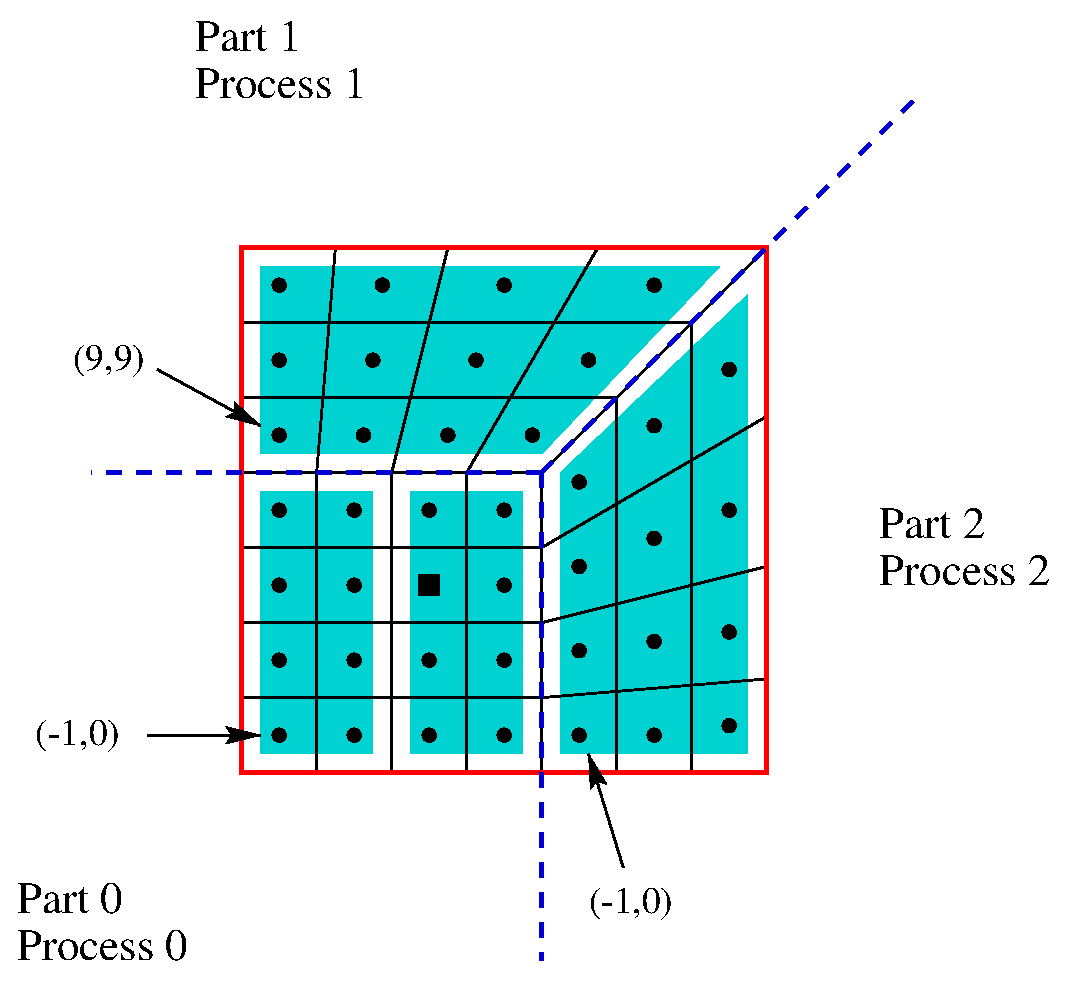
\includegraphics[width=4in]{block_structured.eps}
\caption{%
An example 2D block-structured grid, distributed accross three processes.}
\label{fig-block-structured-grid}
\end{figure}

There are five basic steps involved in setting up the linear system to
be solved:
\begin{itemize}
\item set up the grid,
\item set up the stencils,
\item set up the graph,
\item set up the matrix,
\item set up the right-hand-side vector.
\end{itemize}
To describe each of these steps in more detail, consider solving the
2D Laplacian problem
\begin{equation}\label{sstruct:eqn-laplacian}
\left \{
\begin{array}{ll}
\nabla^2 u = f , & \mbox{in the domain}, \\
u = 0,           & \mbox{on the boundary}.
\end{array}
\right .
\end{equation}
Assume (\ref{eqn-laplacian}) is discretized using standard 9-pt
finite-volumes on the grid pictured in
\ref{fig-block-structured-grid}, and assume that the problem data is
distributed across three processes as depicted.  In the figure, each
grid part is distributed onto a different process, but this need not
be the case; each grid part may also be distributed across several
processes.  Assume for simplicity and illustration that there is a
single coupling between the first and second variables in grid part 0
at index (1,2).  In general, this variable may also be coupled to
variables at neighboring indices.

%==========================================================================

\section{Setting Up the Grid}
\label{sstruct:Setting Up the Grid}

On process 0, the following code will set up the grid shown in the
figure (the code for processes 1 and 2 is similar).
\begin{display}
\begin{verbatim}

HYPRE_SStructGrid     grid;
int                   ilower[2][2] = {{-1, 0}, {1, 0}};
int                   iupper[2][2] = {{ 0, 3}, {2, 3}};
HYPRE_SStructVariable vars[1]      = {HYPRE_SSTRUCT_VARIABLE_CELL};

int                   addindex[2]  = {1,2};
HYPRE_SStructVariable addvars[1]   = {HYPRE_SSTRUCT_VARIABLE_CELL};

HYPRE_SStructGridCreate(MPI_COMM_WORLD, 2, 3, &grid);

HYPRE_SStructGridSetExtents(grid, 0, ilower[0], iupper[0]);
HYPRE_SStructGridSetExtents(grid, 0, ilower[1], iupper[1]);

HYPRE_SStructGridSetVariables(grid, 0, 1, vars);
HYPRE_SStructGridAddVariables(grid, 0, addindex, 1, addvars);

HYPRE_SStructGridAssemble(grid);

\end{verbatim}
\end{display}
The \code{HYPRE_SStructGridCreate()} routine creates an empty 2D grid
object that lives on the \code{MPI_COMM_WORLD} communicator.  The
\code{HYPRE_SStructGridSetExtents()} routine adds a new box to the
grid.  The \code{HYPRE_SStructGridSetVariables()} routine sets the
variables on a grid part, and the
\code{HYPRE_SStructGridAddVariables()} routine adds variables to a grid
part index (in the above example, there are two cell-centered
variables at index (1,2)).  The \code{HYPRE_SStructGridAssemble()}
routine is a collective call (i.e., must be called on all processes),
and finalizes the grid assembly, making the grid ``ready to use''.

%==========================================================================

\section{Setting Up the Stencil}
\label{sstruct:Setting Up the Stencil}

The geometry of the discretization stencil is described by an array of
integer tuples in 2D (triples in 3D), each representing a relative
offset (in index space) from some gridpoint on the grid.  For example,
the geometry of the 9-pt stencil for the example problem being
considered can be represented in the following way:
\begin{equation}\label{sstruct:eqn-stencil-description}
\left [
\begin{array}{ccc}
(-1, 1) & ( 0, 1) & ( 1, 1) \\
(-1, 0) & ( 0, 0) & ( 1, 0) \\
(-1,-1) & ( 0,-1) & ( 1,-1) 
\end{array}
\right ]
\equiv
\left [
\begin{array}{ccc}
S_7 & S_4 & S_8 \\
S_1 & S_0 & S_2 \\
S_5 & S_3 & S_6
\end{array}
\right ] .
\end{equation}
In (\ref{eqn-stencil-description}), the $(0,0)$ entry represents the
``center'' coefficient, and is the 0th entry in the array ($S_0$).
The $(0,-1)$ entry represents the ``south'' coefficient, and is the
3rd entry in the array ($S_3$).  And so on.

On process 0, 1, or 2, the following code will set up the stencil in
(\ref{eqn-stencil-description}).
\begin{display}
\begin{verbatim}

HYPRE_SStructStencil stencil;
int                  s;
int                  offsets[9][2] = {{0,0},
                                      {-1, 0}, { 1, 0}, { 0,-1}, { 0, 1}};
                                      {-1,-1}, {-1, 1}, { 1,-1}, { 1, 1}};

HYPRE_SStructStencilCreate(2, 9, &stencil);

for (s = 0; s < 9; s++)
   HYPRE_SStructStencilSetEntry(stencil, s, offsets[s], 0);

\end{verbatim}
\end{display}
The \code{HYPRE_SStructStencilCreate()} routine creates an empty 2D,
9-pt stencil object.  The \code{HYPRE_SStructStencilSetEntry()}
routine defines the geometry of the stencil, and assigns the array
numbers for each of the stencil entries.  None of the calls are
collective calls.

%==========================================================================

\section{Setting Up the Graph}
\label{sstruct:Setting Up the Graph}

The graph will represent the nonzero structure of the matrix in
Section \ref{sstruct:Setting Up the Matrix} below.  It is defined in
terms of the grid and stencil objects described in Sections
\ref{sstruct:Setting Up the Grid} and \ref{sstruct:Setting Up the
Stencil} above.

On process 0, the following code will set up the graph for the
example problem.
\begin{display}
\begin{verbatim}

HYPRE_SStructGraph graph;
int                addindex[8][2]   = {{ 2,0},{2,1},{2,2},{2,3},
                                       {-1,3},{0,3},{1,3},
                                       { 1,2}};
int                addentries[9][2] = {{-1,0},{-1,1},{-1,2},{-1,3},
                                       { 9,9},{10,9},{11,9},{12,9},
                                       { 1,2}};

HYPRE_SStructGraphCreate(MPI_COMM_WORLD, grid, &graph);

HYPRE_SStructGraphSetStencil(graph, 0, 0, stencil);

/* Add graph edge entries at grid part boundaries */
HYPRE_SStructGraphAddEntries(graph, 0, addindex[0], 0, 2, 2, &addentries[0], 0);
HYPRE_SStructGraphAddEntries(graph, 0, addindex[1], 0, 3, 2, &addentries[0], 0);
HYPRE_SStructGraphAddEntries(graph, 0, addindex[2], 0, 3, 2, &addentries[1], 0);
...

/* Add graph edge entries at index (1,2) */
HYPRE_SStructGraphAddEntries(graph, 0, addindex[7], 0, 1, 0, &addentries[8], 1);
HYPRE_SStructGraphAddEntries(graph, 0, addindex[7], 1, 1, 0, &addentries[8], 0);

\end{verbatim}
\end{display}

%==========================================================================

\section{Setting Up the Matrix}
\label{sstruct:Setting Up the Matrix}

The matrix is set up in terms of the graph object described in Section
\ref{sstruct:Setting Up the Graph} above.  The coefficients associated
with each graph entry will typically vary from gridpoint to gridpoint,
but in the example problem being considered, they are as follows over
the entire grid (except at boundaries; see below):
\begin{equation}\label{sstruct:eqn-stencil-laplacian}
\left [
\begin{array}{ccc}
 -1 & -1 & -1 \\
 -1 &  8 & -1 \\
 -1 & -1 & -1 
\end{array}
\right ] .
\end{equation}

On process 0, the following code will set up matrix values associated
with the center ($S_0$) and south ($S_3$) stencil entries in
(\ref{eqn-stencil-description}) / (\ref{eqn-stencil-laplacian}).
Matrix values associated with the non-stencil graph entries are also
set up.
\begin{display}
\begin{verbatim}

HYPRE_SStructMatrix  A;
double               values[32];
int                  sindices[2] = {0,3};
int                  gindices[2] = {9,10,11,0};
int                  i;

HYPRE_SStructMatrixCreate(MPI_COMM_WORLD, graph, &A);
HYPRE_SStructMatrixInitialize(A);

for (i = 0; i < 32; i += 2)
{
   values[i]   =  8.0;
   values[i+1] = -1.0;
}
HYPRE_SStructMatrixSetBoxValues(A, 0, ilower[0], iupper[0], 0,
                                2, sindices, values);

/* set values at non-stencil graph entries */
for (i = 0; i < 3; i++)
{
   values[i] = -1.0;
}
HYPRE_SStructMatrixSetValues(A, 0, addindex[0], 0, 2, gindices, values);
HYPRE_SStructMatrixSetValues(A, 0, addindex[1], 0, 3, gindices, values);
HYPRE_SStructMatrixSetValues(A, 0, addindex[2], 0, 3, gindices, values);
...
HYPRE_SStructMatrixSetValues(A, 0, addindex[7], 0, 1, gindices, values);
HYPRE_SStructMatrixSetValues(A, 0, addindex[7], 1, 1, &gindices[3], values);

/* zero out coefficients that reach outside of the domain or grid part */
...

/* set boundary conditions at domain boundaries, */
...

HYPRE_SStructMatrixAssemble(A);

\end{verbatim}
\end{display}

%==========================================================================

\section{Setting Up the Right-Hand-Side Vector}
\label{sstruct:Setting Up the Right-Hand-Side Vector}

The right-hand-side vector is set up similarly to the matrix set up
described in Section \ref{sstruct:Setting Up the Matrix} above.  The
main difference is that there is no graph.

%==========================================================================

